\documentclass[10pt,]{krantz}
\usepackage{lmodern}
\usepackage{amssymb,amsmath}
\usepackage{ifxetex,ifluatex}
\usepackage{fixltx2e} % provides \textsubscript
\ifnum 0\ifxetex 1\fi\ifluatex 1\fi=0 % if pdftex
  \usepackage[T1]{fontenc}
  \usepackage[utf8]{inputenc}
\else % if luatex or xelatex
  \ifxetex
    \usepackage{mathspec}
  \else
    \usepackage{fontspec}
  \fi
  \defaultfontfeatures{Ligatures=TeX,Scale=MatchLowercase}
\fi
% use upquote if available, for straight quotes in verbatim environments
\IfFileExists{upquote.sty}{\usepackage{upquote}}{}
% use microtype if available
\IfFileExists{microtype.sty}{%
\usepackage{microtype}
\UseMicrotypeSet[protrusion]{basicmath} % disable protrusion for tt fonts
}{}
\usepackage[unicode=true]{hyperref}
\PassOptionsToPackage{usenames,dvipsnames}{color} % color is loaded by hyperref
\hypersetup{
            pdftitle={Manual de R},
            colorlinks=true,
            linkcolor=Maroon,
            citecolor=Blue,
            urlcolor=Blue,
            breaklinks=true}
\urlstyle{same}  % don't use monospace font for urls
\usepackage{natbib}
\bibliographystyle{apalike}
\usepackage{color}
\usepackage{fancyvrb}
\newcommand{\VerbBar}{|}
\newcommand{\VERB}{\Verb[commandchars=\\\{\}]}
\DefineVerbatimEnvironment{Highlighting}{Verbatim}{commandchars=\\\{\}}
% Add ',fontsize=\small' for more characters per line
\usepackage{framed}
\definecolor{shadecolor}{RGB}{248,248,248}
\newenvironment{Shaded}{\begin{snugshade}}{\end{snugshade}}
\newcommand{\KeywordTok}[1]{\textcolor[rgb]{0.13,0.29,0.53}{\textbf{{#1}}}}
\newcommand{\DataTypeTok}[1]{\textcolor[rgb]{0.13,0.29,0.53}{{#1}}}
\newcommand{\DecValTok}[1]{\textcolor[rgb]{0.00,0.00,0.81}{{#1}}}
\newcommand{\BaseNTok}[1]{\textcolor[rgb]{0.00,0.00,0.81}{{#1}}}
\newcommand{\FloatTok}[1]{\textcolor[rgb]{0.00,0.00,0.81}{{#1}}}
\newcommand{\ConstantTok}[1]{\textcolor[rgb]{0.00,0.00,0.00}{{#1}}}
\newcommand{\CharTok}[1]{\textcolor[rgb]{0.31,0.60,0.02}{{#1}}}
\newcommand{\SpecialCharTok}[1]{\textcolor[rgb]{0.00,0.00,0.00}{{#1}}}
\newcommand{\StringTok}[1]{\textcolor[rgb]{0.31,0.60,0.02}{{#1}}}
\newcommand{\VerbatimStringTok}[1]{\textcolor[rgb]{0.31,0.60,0.02}{{#1}}}
\newcommand{\SpecialStringTok}[1]{\textcolor[rgb]{0.31,0.60,0.02}{{#1}}}
\newcommand{\ImportTok}[1]{{#1}}
\newcommand{\CommentTok}[1]{\textcolor[rgb]{0.56,0.35,0.01}{\textit{{#1}}}}
\newcommand{\DocumentationTok}[1]{\textcolor[rgb]{0.56,0.35,0.01}{\textbf{\textit{{#1}}}}}
\newcommand{\AnnotationTok}[1]{\textcolor[rgb]{0.56,0.35,0.01}{\textbf{\textit{{#1}}}}}
\newcommand{\CommentVarTok}[1]{\textcolor[rgb]{0.56,0.35,0.01}{\textbf{\textit{{#1}}}}}
\newcommand{\OtherTok}[1]{\textcolor[rgb]{0.56,0.35,0.01}{{#1}}}
\newcommand{\FunctionTok}[1]{\textcolor[rgb]{0.00,0.00,0.00}{{#1}}}
\newcommand{\VariableTok}[1]{\textcolor[rgb]{0.00,0.00,0.00}{{#1}}}
\newcommand{\ControlFlowTok}[1]{\textcolor[rgb]{0.13,0.29,0.53}{\textbf{{#1}}}}
\newcommand{\OperatorTok}[1]{\textcolor[rgb]{0.81,0.36,0.00}{\textbf{{#1}}}}
\newcommand{\BuiltInTok}[1]{{#1}}
\newcommand{\ExtensionTok}[1]{{#1}}
\newcommand{\PreprocessorTok}[1]{\textcolor[rgb]{0.56,0.35,0.01}{\textit{{#1}}}}
\newcommand{\AttributeTok}[1]{\textcolor[rgb]{0.77,0.63,0.00}{{#1}}}
\newcommand{\RegionMarkerTok}[1]{{#1}}
\newcommand{\InformationTok}[1]{\textcolor[rgb]{0.56,0.35,0.01}{\textbf{\textit{{#1}}}}}
\newcommand{\WarningTok}[1]{\textcolor[rgb]{0.56,0.35,0.01}{\textbf{\textit{{#1}}}}}
\newcommand{\AlertTok}[1]{\textcolor[rgb]{0.94,0.16,0.16}{{#1}}}
\newcommand{\ErrorTok}[1]{\textcolor[rgb]{0.64,0.00,0.00}{\textbf{{#1}}}}
\newcommand{\NormalTok}[1]{{#1}}
\usepackage{longtable,booktabs}
\IfFileExists{parskip.sty}{%
\usepackage{parskip}
}{% else
\setlength{\parindent}{0pt}
\setlength{\parskip}{6pt plus 2pt minus 1pt}
}
\setlength{\emergencystretch}{3em}  % prevent overfull lines
\providecommand{\tightlist}{%
  \setlength{\itemsep}{0pt}\setlength{\parskip}{0pt}}
\setcounter{secnumdepth}{5}
% Redefines (sub)paragraphs to behave more like sections
\ifx\paragraph\undefined\else
\let\oldparagraph\paragraph
\renewcommand{\paragraph}[1]{\oldparagraph{#1}\mbox{}}
\fi
\ifx\subparagraph\undefined\else
\let\oldsubparagraph\subparagraph
\renewcommand{\subparagraph}[1]{\oldsubparagraph{#1}\mbox{}}
\fi
\usepackage{booktabs}
\usepackage[spanish]{babel}
\decimalpoint
\selectlanguage{spanish}

% Comandos para escribir nombres de paquetes, programas y codigos
\newcommand{\pkg}[1]{{\normalfont\fontseries{b}\selectfont #1}}
\let\proglang=\textsf
\let\code=\texttt


\usepackage{booktabs}
\usepackage{longtable}
\usepackage[bf,singlelinecheck=off]{caption}

\usepackage{framed,color}
\definecolor{shadecolor}{RGB}{248,248,248}

\renewcommand{\textfraction}{0.05}
\renewcommand{\topfraction}{0.8}
\renewcommand{\bottomfraction}{0.8}
\renewcommand{\floatpagefraction}{0.75}

\renewenvironment{quote}{\begin{VF}}{\end{VF}}
\let\oldhref\href
\renewcommand{\href}[2]{#2\footnote{\url{#1}}}

\ifxetex
  \usepackage{letltxmacro}
  \setlength{\XeTeXLinkMargin}{1pt}
  \LetLtxMacro\SavedIncludeGraphics\includegraphics
  \def\includegraphics#1#{% #1 catches optional stuff (star/opt. arg.)
    \IncludeGraphicsAux{#1}%
  }%
  \newcommand*{\IncludeGraphicsAux}[2]{%
    \XeTeXLinkBox{%
      \SavedIncludeGraphics#1{#2}%
    }%
  }%
\fi

\makeatletter
\newenvironment{kframe}{%
\medskip{}
\setlength{\fboxsep}{.8em}
 \def\at@end@of@kframe{}%
 \ifinner\ifhmode%
  \def\at@end@of@kframe{\end{minipage}}%
  \begin{minipage}{\columnwidth}%
 \fi\fi%
 \def\FrameCommand##1{\hskip\@totalleftmargin \hskip-\fboxsep
 \colorbox{shadecolor}{##1}\hskip-\fboxsep
     % There is no \\@totalrightmargin, so:
     \hskip-\linewidth \hskip-\@totalleftmargin \hskip\columnwidth}%
 \MakeFramed {\advance\hsize-\width
   \@totalleftmargin\z@ \linewidth\hsize
   \@setminipage}}%
 {\par\unskip\endMakeFramed%
 \at@end@of@kframe}
\makeatother

\renewenvironment{Shaded}{\begin{kframe}}{\end{kframe}}

\usepackage{makeidx}
\makeindex

\urlstyle{tt}

\usepackage{amsthm}
\makeatletter
\def\thm@space@setup{%
  \thm@preskip=8pt plus 2pt minus 4pt
  \thm@postskip=\thm@preskip
}
\makeatother

\frontmatter

\title{Manual de R}
\author{Freddy Hernández Barajas\\
Olga Cecilia Usuga Manco}
\date{2017-01-18}

\let\BeginKnitrBlock\begin \let\EndKnitrBlock\end
\begin{document}
\maketitle

% you may need to leave a few empty pages before the dedication page

%\cleardoublepage\newpage\thispagestyle{empty}\null
%\cleardoublepage\newpage\thispagestyle{empty}\null
%\cleardoublepage\newpage
\thispagestyle{empty}

\begin{center}

Gracias a Dios por todo lo que me ha dado.

%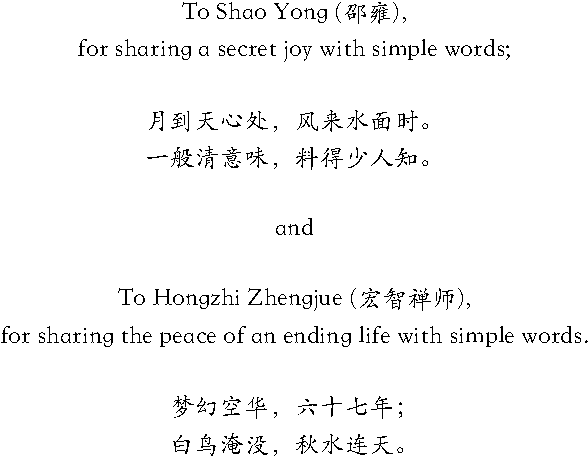
\includegraphics{images/dedication.pdf}
\end{center}

\setlength{\abovedisplayskip}{-5pt}
\setlength{\abovedisplayshortskip}{-5pt}

{
\hypersetup{linkcolor=black}
\setcounter{tocdepth}{2}
\tableofcontents
}
\listoftables
\listoffigures
\chapter*{Prefacio}\label{prefacio}


Este libro fue creado con la intención de \ldots{}

\section*{¿Por qué leer este libro?}\label{por-que-leer-este-libro}


Este libro es importante porque \ldots{}

\section*{Estructura del libro}\label{estructura-del-libro}


En el capítulo \ref{Introducción} se presenta una introducción breve de
\proglang{R}, sus orígenes, la instalación, tipos de objetos y una guía
de estilo para escribir en \proglang{R}.

\section*{Software information and
conventions}\label{software-information-and-conventions}


Para realizar este libro usamos los paquetes \textbf{knitr}\index{knitr}
\citep{xie2015} y \textbf{bookdown}\index{bookdown} \citep{R-bookdown}.
La información de la sesión de \proglang{R} usada se muestra abajo:

\begin{Shaded}
\begin{Highlighting}[]
\KeywordTok{sessionInfo}\NormalTok{()}
\end{Highlighting}
\end{Shaded}

\begin{verbatim}
## R version 3.3.2 (2016-10-31)
## Platform: x86_64-w64-mingw32/x64 (64-bit)
## Running under: Windows 7 x64 (build 7601) Service Pack 1
## 
## locale:
## [1] LC_COLLATE=English_Australia.1252 
## [2] LC_CTYPE=English_Australia.1252   
## [3] LC_MONETARY=English_Australia.1252
## [4] LC_NUMERIC=C                      
## [5] LC_TIME=English_Australia.1252    
## 
## attached base packages:
## [1] stats     graphics  grDevices utils     datasets 
## [6] methods   base     
## 
## loaded via a namespace (and not attached):
##  [1] backports_1.0.4 bookdown_0.3    magrittr_1.5   
##  [4] rprojroot_1.1   tools_3.3.2     htmltools_0.3.5
##  [7] rstudioapi_0.6  yaml_2.1.14     Rcpp_0.12.8    
## [10] stringi_1.1.2   rmarkdown_1.3   knitr_1.15.1   
## [13] stringr_1.1.0   digest_0.6.11   evaluate_0.10
\end{verbatim}

Package names are in bold text (e.g., \textbf{rmarkdown}), and inline
code and filenames are formatted in a typewriter font (e.g.,
\texttt{knitr::knit(\textquotesingle{}foo.Rmd\textquotesingle{})}).
Function names are followed by parentheses (e.g.,
\texttt{bookdown::render\_book()}).

\section*{Agradecimientos}\label{agradecimientos}


Agradecemos a \ldots{}

\BeginKnitrBlock{flushright}
Freddy Hernández Barajas Olga Cecilia Usuga Manco
\EndKnitrBlock{flushright}

\chapter*{Sobre los autores}\label{sobre-los-autores}


Freddy Hernández Barajas es profesor asistente de la Universidad
Nacional de Colombia adscrito a la Escuela de Estadística de la Facultad
de Ciencias.

Olga Cecilia Usuga Manco es profesora asociado de la Universidad de
Antioquia adscrita a la Facultad de Ingeniería.

\cleardoublepage 

\appendix \addcontentsline{toc}{chapter}{\appendixname}


\chapter{More to Say}\label{more-to-say}

Yeah! I have finished my book, but I have more to say about some topics.
Let me explain them in this appendix.

To know more about \textbf{bookdown}, see \url{https://bookdown.org}.

\bibliography{packages,book}

\backmatter
\printindex

\end{document}
